% Options for packages loaded elsewhere
\PassOptionsToPackage{unicode}{hyperref}
\PassOptionsToPackage{hyphens}{url}
%
\documentclass[
]{article}
\usepackage{amsmath,amssymb}
\usepackage{lmodern}
\usepackage{iftex} 
\ifPDFTeX
  \usepackage[T1]{fontenc}
  \usepackage[utf8]{inputenc}
  \usepackage{textcomp} % provide euro and other symbols
\else % if luatex or xetex
  \usepackage{unicode-math}
  \defaultfontfeatures{Scale=MatchLowercase}
  \defaultfontfeatures[\rmfamily]{Ligatures=TeX,Scale=1}
\fi
% Use upquote if available, for straight quotes in verbatim environments
\IfFileExists{upquote.sty}{\usepackage{upquote}}{}
\IfFileExists{microtype.sty}{% use microtype if available
  \usepackage[]{microtype}
  \UseMicrotypeSet[protrusion]{basicmath} % disable protrusion for tt fonts
}{}
\makeatletter
\@ifundefined{KOMAClassName}{% if non-KOMA class
  \IfFileExists{parskip.sty}{%
    \usepackage{parskip}
  }{% else
    \setlength{\parindent}{0pt}
    \setlength{\parskip}{6pt plus 2pt minus 1pt}}
}{% if KOMA class
  \KOMAoptions{parskip=half}}
\makeatother
\usepackage{xcolor}
\usepackage{color}
\usepackage{fancyvrb} 
\newcommand{\VerbBar}{|}
\newcommand{\VERB}{\Verb[commandchars=\\\{\}]}
\DefineVerbatimEnvironment{Highlighting}{Verbatim}{commandchars=\\\{\}}
% Add ',fontsize=\small' for more characters per line
\newenvironment{Shaded}{}{}
\newcommand{\AlertTok}[1]{\textcolor[rgb]{1.00,0.00,0.00}{\textbf{#1}}}
\newcommand{\AnnotationTok}[1]{\textcolor[rgb]{0.38,0.63,0.69}{\textbf{\textit{#1}}}}
\newcommand{\AttributeTok}[1]{\textcolor[rgb]{0.49,0.56,0.16}{#1}}
\newcommand{\BaseNTok}[1]{\textcolor[rgb]{0.25,0.63,0.44}{#1}}
\newcommand{\BuiltInTok}[1]{\textcolor[rgb]{0.00,0.50,0.00}{#1}}
\newcommand{\CharTok}[1]{\textcolor[rgb]{0.25,0.44,0.63}{#1}}
\newcommand{\CommentTok}[1]{\textcolor[rgb]{0.38,0.63,0.69}{\textit{#1}}}
\newcommand{\CommentVarTok}[1]{\textcolor[rgb]{0.38,0.63,0.69}{\textbf{\textit{#1}}}}
\newcommand{\ConstantTok}[1]{\textcolor[rgb]{0.53,0.00,0.00}{#1}}
\newcommand{\ControlFlowTok}[1]{\textcolor[rgb]{0.00,0.44,0.13}{\textbf{#1}}}
\newcommand{\DataTypeTok}[1]{\textcolor[rgb]{0.56,0.13,0.00}{#1}}
\newcommand{\DecValTok}[1]{\textcolor[rgb]{0.25,0.63,0.44}{#1}}
\newcommand{\DocumentationTok}[1]{\textcolor[rgb]{0.73,0.13,0.13}{\textit{#1}}}
\newcommand{\ErrorTok}[1]{\textcolor[rgb]{1.00,0.00,0.00}{\textbf{#1}}}
\newcommand{\ExtensionTok}[1]{#1}
\newcommand{\FloatTok}[1]{\textcolor[rgb]{0.25,0.63,0.44}{#1}}
\newcommand{\FunctionTok}[1]{\textcolor[rgb]{0.02,0.16,0.49}{#1}}
\newcommand{\ImportTok}[1]{\textcolor[rgb]{0.00,0.50,0.00}{\textbf{#1}}}
\newcommand{\InformationTok}[1]{\textcolor[rgb]{0.38,0.63,0.69}{\textbf{\textit{#1}}}}
\newcommand{\KeywordTok}[1]{\textcolor[rgb]{0.00,0.44,0.13}{\textbf{#1}}}
\newcommand{\NormalTok}[1]{#1}
\newcommand{\OperatorTok}[1]{\textcolor[rgb]{0.40,0.40,0.40}{#1}}
\newcommand{\OtherTok}[1]{\textcolor[rgb]{0.00,0.44,0.13}{#1}}
\newcommand{\PreprocessorTok}[1]{\textcolor[rgb]{0.74,0.48,0.00}{#1}}
\newcommand{\RegionMarkerTok}[1]{#1}
\newcommand{\SpecialCharTok}[1]{\textcolor[rgb]{0.25,0.44,0.63}{#1}}
\newcommand{\SpecialStringTok}[1]{\textcolor[rgb]{0.73,0.40,0.53}{#1}}
\newcommand{\StringTok}[1]{\textcolor[rgb]{0.25,0.44,0.63}{#1}}
\newcommand{\VariableTok}[1]{\textcolor[rgb]{0.10,0.09,0.49}{#1}}
\newcommand{\VerbatimStringTok}[1]{\textcolor[rgb]{0.25,0.44,0.63}{#1}}
\newcommand{\WarningTok}[1]{\textcolor[rgb]{0.38,0.63,0.69}{\textbf{\textit{#1}}}}
\usepackage{graphicx}
\makeatletter
\def\maxwidth{\ifdim\Gin@nat@width>\linewidth\linewidth\else\Gin@nat@width\fi}
\def\maxheight{\ifdim\Gin@nat@height>\textheight\textheight\else\Gin@nat@height\fi}
\makeatother
% Scale images if necessary, so that they will not overflow the page
% margins by default, and it is still possible to overwrite the defaults
% using explicit options in \includegraphics[width, height, ...]{}
\setkeys{Gin}{width=\maxwidth,height=\maxheight,keepaspectratio}
% Set default figure placement to htbp
\makeatletter
\def\fps@figure{htbp}
\makeatother
\setlength{\emergencystretch}{3em} % prevent overfull lines
\providecommand{\tightlist}{%
  \setlength{\itemsep}{0pt}\setlength{\parskip}{0pt}}
\setcounter{secnumdepth}{-\maxdimen} % remove section numbering
\ifLuaTeX
  \usepackage{selnolig}  % disable illegal ligatures
\fi
\usepackage[]{biblatex}
\IfFileExists{bookmark.sty}{\usepackage{bookmark}}{\usepackage{hyperref}}
\IfFileExists{xurl.sty}{\usepackage{xurl}}{} % add URL line breaks if available
\urlstyle{same} % disable monospaced font for URLs
\hypersetup{
  hidelinks,
  pdfcreator={LaTeX via pandoc}}

\author{}
\date{}

\begin{document}

The field of Secure Multiparty Computation provides methods for jointly
computing functions without revealing their private inputs from multple
parties. This master thesis assignment focuses on the MPyC framework for
MPC and explores various approaches for connecting the parties via the
internet. A technical survey was performed in the preparation phase to
identify viable techniques and tools to achieve that. Furthermore a test
environment dubbed \(E^3\) was developed to support the exploration
process that will take place during the implementation phase of the
assignment. It is composed of a combination of physical and virtual
machines that are able to execute a multiparty computation together
using MPyC. It employs several declarative Infrastructure as Code tools
to automate the deployment process and make it reproducible.
Specifically, Terraform is used for provisioning NixOS virtual machines
on the DigitalOcean cloud provider and Colmena is used for remotely
deploying software to them. The reference implementation described in
this report uses the Tailscale mesh VPN for connectivity, and a number
of additional implementations are planned for the next phase of the
project.

\hypertarget{introduction}{%
  \section{Introduction}\label{introduction}}

This report will present the results of the preparation phase of the
master thesis project titled ``Secure Sessions for Ad Hoc Multiparty
Computation in MPyC''. The goal of this phase is to gain sufficient
insight into the topic, perform some preliminary tasks and propose a
plan with well defined goals for the implementation phase of the
project.

\hypertarget{background}{%
  \subsection{Background}\label{background}}

\gls{mpc} is a set of techniques and protocols for computing a function
over the secret inputs of multiple parties without revealing their
values, but only the final result. A good overview can be found on
Wikipedia\autocite{wikiMPC}. Yao's Millionaires'
Problem\autocite{yaoProtocolsSecureComputations1982} is one famous
example in which a number of millionaires want to know who is richer
without revealing their net worths. Other practical
applications\autocite{laudApplicationsSecureMultiparty2015} include
electronic voting, auctions or even machine
learning\autocite{knottCrypTenSecureMultiParty2022} where one party's
private data can be used as an input for another party's private machine
learning model.

The general process is that each party uses a scheme like \gls{sss}
\autocite{shamirHowShareSecret1979} to split its secret input into
shares and sends one to each of the other parties. A protocol involving
multiple communication rounds and further re-shares of intermediate
secret results is used by the parties so that each of them can compute
the final result from the shares it has received.

A number of \gls{mpc} frameworks have been developed for various
programming languages and security models. As part of this project we
will focus our efforts on \textbf{MPyC}\autocite{mpycHome,mpycSource} -
an opensource \gls{mpc} Python framework developed primarily at TU
Eindhoven, but our results should be applicable to others as well.

To help us determine the types of solutions we need to consider, we can
group the potential users of the MPyC framework into three broad
categories: casual users, power users and enterprises.

We define \textbf{casual users} as people who are used to Windows or
Mac, prefer software installers to package managers, \gls{gui} programs
rather than \gls{cli} based ones and do not feel comfortable with
manually modifying their systems or using scripts.

We define \textbf{power users} as users who manage a number of personal
physical machines and may have some familiarity with Linux, terminals
and shell scripting. They are assumed to be able to execute the
necessary steps to setup a machine given a guide.

For our purposes we define \textbf{enterprises} as companies with
operations departments that manage their IT infrastructure and optimize
for scale. They usually have large numbers of Linux based servers which
are a combination of physical, virtual and container based. Those can be
deployed either in the cloud or on premise in an automated way using
\gls{iac} tools.

\hypertarget{problem-description}{%
  \subsection{Problem description}\label{problem-description}}

MPyC supports \gls{tcp} connections from the \gls{ip} suite between the
\gls{mpc} participants but it does not currently provide a service
discovery mechanism. Before performing a joint computation, all parties
must know and be able to reach each other's \gls{tcp} endpoints - either
via a local \gls{ip} address on a \gls{lan}, or via a public \gls{ip}
address or the \gls{dns} on the internet. This is not likely to pose a
problem for most enterprise users, who are usually already exposing some
public services, e.g.~their website. However, most casual users who are
not \gls{it} experts typically do not own a domain name nor know how to
configure a publicly accessible server. Due to the limited supply of
addresses supported by \gls{ip}v4 and the slow adoption of \gls{ip}v6,
most \glspl{isp} do not allocate a public address for each machine in
the home networks of their residential customers. Usually only their
router has a temporary public address and it utilizes techniques such as
\gls{nat} in order to enable the other local machines to initiate remote
internet connections. However, connections to them cannot be initiated
from outside the \gls{lan} without manually configuring port forwarding
in the router to send the appropriate traffic to the intended machine.
This poses some challenges and limits the usability of MPyC in every day
scenarios due to the inherently \gls{p2p} nature of the involved
communications.

\hypertarget{research-questions}{%
  \subsection{Research questions}\label{research-questions}}

Based on the problem description above, we formulate the following
central research question:

\emph{How can MPyC be extended to enable casual users, power users and
  enterprises with limited prior knowledge of each other to discover each
  other and perform a secure multiparty computation under diverse
  networking conditions?}

We further identify the following sub-questions:

\begin{itemize}
  \tightlist
  \item
        \emph{What deployment strategies should be supported in order to
          accommodate the potential users of MPyC programs?}
\end{itemize}

Depending on the technical background of a user and their typical
computing usage, they might have different expectations for how to
execute their part of the joint multiparty computation, e.g.~enterprises
might expect support for automation tools, while casual users could
expect simplicity. There should be some safety (not necessarily
security) mechanism for detecting and preventing mistakes where the
users are accidentally executing incompatible MPyC programs/versions.

\begin{itemize}
  \tightlist
  \item
        \emph{What are the most suitable approaches for a party to obtain an
          identity and prove it to other parties for the purposes of MPC?}
\end{itemize}

A party's digital identity is a persistent mechanism that allows others
to provably track it across digital interactions with the party. An
identity can either be issued by a digital authority, e.g.~an
organization like google, or a country's government or it can be
self-issued. Depending on the method, an identity verification can
involve demonstrating a cryptographic proof of ownership of a public
key, or separate communication with the digital authority.

\begin{itemize}
  \tightlist
  \item
        \emph{What mechanisms can be used by the parties to initially get in
          contact and discover each other's identities?}
\end{itemize}

Different approaches should be considered based on the types of users
and their prior relationships. Some examples could be for companies to
publicly post their identities on their websites, end-users who know
each other could use social media or group chats and if they do not know
each other, they could use an (anonymous) matchmaking service.

\begin{itemize}
  \tightlist
  \item
        \emph{How can the parties establish communication channels with each
          other based on the chosen identity solutions under diverse networking
          conditions?}
\end{itemize}

As previously mentioned, some parties could be on a home network and not
have a public \gls{ip}, which may require considering approaches that
use a mediator.

\begin{itemize}
  \tightlist
  \item
        \emph{How can the parties communicate securely as part of the MPC
          execution? To what extent can the parties' privacy be preserved? How
          efficiently can this be achieved?}
\end{itemize}

In order for the execution of an \gls{mpc} protocol to be secure, it is
important for the parties to be able to cryptographically verify the
identity of a message's original sender and be certain that nobody other
than themselves can read it. Solutions that do not reveal physically
identifying information such as \gls{ip} addresses are also interesting
to consider. The performance overhead of the security mechanisms should
be evaluated.

\hypertarget{preparation-phase-scope}{%
  \subsection{Preparation phase scope}\label{preparation-phase-scope}}

During the implementation phase, we will answer the posed research
questions of the project after evaluating various connectivity
approaches for MPyC. The scope of the preparation phase will cover a
technical survey to identify some of the tools that can be used and the
development of an \gls{e3} that will support the evaluation process in
the next phase. \gls{e3} must enable fearless experimentation with
different implementations of the connectivity layer. \gls{e3} will focus
on being reproducible by enterprise and power users while keeping it
representative of real world scenarios involving casual users as well.

Below, we formulate our requirements for \gls{e3} and group them in
terms of several important characteristics:

\begin{itemize}
  \tightlist
  \item
        Complexity

        \begin{itemize}
          \tightlist
          \item
                simple - given the limited time of the preparation phase, \gls{e3}
                must focus on simplicity, e.g.~the easiest to implement connectivity
                approach should be chosen
          \item
                extensible - \gls{e3} must allow for switching the building blocks
                during the next phase of the project, e.g.~it should be easy to
                experiment with different connectivity approaches in order to
                measure and compare their characteristics
        \end{itemize}
  \item
        Source code

        \begin{itemize}
          \tightlist
          \item
                open-source - the source code of the resulting implementation of
                \gls{e3} must be available in a public repository, e.g.~on
                Github.com
          \item
                no plaintext secrets such as \gls{api} keys and passwords should be
                present in the public repository, but others should be able to
                easily provide their own secrets in order to use \gls{e3} in their
                own environment.
        \end{itemize}
  \item
        Deployment

        \begin{itemize}
          \tightlist
          \item
                cross region - the machines should be provisioned in multiple
                geographical regions in order to be able to observe the effects of
                varying latency on the system
          \item
                cross platform - in a real world scenario the machines will be
                controlled by different parties that run various operating systems,
                hardware architectures and deployed using different tools,
                e.g.~Party A might be an enterprise that uses containers, while
                Party B is a power user running a few \glspl{vm} and Party C
                ****could be using an ARM-based raspberry pi
          \item
                automated - appropriate tools should be chosen to allow
                automatically deploying and destroying the runtime environment
                without manual intervention other than running a minimal set of
                commands
          \item
                reproducible - it should be easy for others to reproduce the test
                setup in their own environment
          \item
                disposable - \gls{e3} should be easy to destroy and quickly recreate
                from scratch at any time; as in the famous DevOps
                analogy\autocite{biasHistoryPetsVs2016}, it should be based on
                machines that are like cattle rather than pets
        \end{itemize}
  \item
        Connectivity

        \begin{itemize}
          \tightlist
          \item
                identity - it must be possible for the machines to communicate based
                on a long-lived identity rather than a potentially temporary
                \gls{ip} address.
          \item
                secure - a message sent by a party must be readable only by its
                intended targets.
          \item
                authenticated - a party must be able to determine which party a
                message was sent by
          \item
                private - no more information than strictly necessary should be
                revealed about a party. Depending on the method of communication, it
                may be necessary to choose a tradeoff or introduce a tuning
                parameter between performance and privacy.
        \end{itemize}
\end{itemize}

\hypertarget{goals}{%
  \section{Goals}\label{goals}}

\hypertarget{motivation}{%
  \subsection{Motivation}\label{motivation}}

\hypertarget{technical-survey}{%
  \section{Technical Survey}\label{technical-survey}}

In this chapter we will perform a high level survey of the available
tools and approaches that could be used for \gls{e3} and select ones
that fit our requirements. In the next chapter we will go more in depth
and cover the implementation details using those tools.

Since we need to design for a heterogeneous runtime environment, we need
to choose building blocks that are compatible with as many scenarios as
possible while also keeping the complexity low.

\hypertarget{deployment}{%
  \subsection{Deployment}\label{deployment}}

Our primary users are enterprises and power users. Enterprises can
employ a variety of \gls{iac} tools in their infrastructure management
process:

\begin{itemize}
  \tightlist
  \item
        provisioning - Terraform\autocite{tfDocs}, Cloud
        Formation\autocite{cfDocs}, etc.
  \item
        deployment automation - Ansible\autocite{ansibleDocs},
        Puppet\autocite{puppetDocs}, Chef\autocite{chefDocs}, etc.
  \item
        container orchestration - Docker Swarm\autocite{dockerDocs},
        Kubernetes\autocite{kubeDocs}, etc.
\end{itemize}

According to our definitions, power users typically use physical
machines while enterprises can use both virtual machines and container
orchestration tools. Based on our requirements for \gls{e3} we need a
cross region deployment. \glspl{vm} can be automatically provisioned
across different regions in the cloud using \gls{iac} tools. Once
provisioned, a \gls{vm} is usually managed via an automation tool that
executes a set of deployment steps over SSH. Those deployment steps can
be adapted to physical machines so that power users can make use of
them.

Kubernetes is used for dynamically scaling a large number of
long-running processes across a cluster of \glspl{vm} within the same
geographic region. Enterprises may wish to run MPyC programs in a
Kubernetes cluster and might benefit from an example of doing so. But
for the purposes of \gls{e3}, it does not provide sufficient benefits
compared to using \glspl{vm} directly, while it adds complexity in terms
of deploying multiple clusters across regions and adding a cross cluster
communication mechanism.

Based on this analysis, we choose to base \gls{e3} on a combination of
\glspl{vm} deployed in the cloud and a set of personal devices owned by
the authors - a Linux laptop, a Windows desktop with Windows Subsystem
for Linux, and an ARM Raspberry Pi 2 to serve as an example of both
enterprises and individual power users.

\gls{iac} tools use specifications that are either imperative or
declarative. \textbf{Imperative} specifications describe the steps
needed to be executed for the infrastructure to reach the desired state,
while \textbf{declarative} specifications describe the desired final
state and let the tool worry about how to get there. Imperative tools
are more likely to suffer from \emph{configuration drift} - the
infrastructure state might become out of sync with the specification due
to either manual changes or left-over state from previously applied
specifications. On the other hand, if something is removed from a
declarative specification, when it gets applied, the corresponding
resources will also be removed from the infrastructure. In addition,
declarative tools are idempotent - applying the same specification
multiple times in a row does not change the state. Therefore in order to
achieve high reproducibility, we will prefer declarative tools to
imperative ones where possible.

On Linux, software is usually installed via package managers. Most of
the popular Linux distributions such as Ubuntu, Debian, Fedora, Arch use
package managers that only support automating this process via
imperative shell scripts rather than a declarative specification.
Additionally those do not offer an easy way of specifying and locking
the required software versions to a known good configuration that can be
reproduced in the future. NixOS on the other hand is based on the
declarative Nix package manager which does support version locking via
its \textbf{flakes} feature. This is why we choose to use the NixOS
operating system for our \glspl{vm}.

Most of the popular application deployment tools such as Ansible, Chef
and Puppet are either imperative or have limited support for declarative
specifications. Fortunately, the NixOS ecosystem, offers a number of
deployment tools that can apply a declarative specification on remote
hosts:

\begin{itemize}
  \tightlist
  \item
        NixOps\autocite{nixopsSource,nixopsDocs} - official tool
  \item
        Colmena \autocite{colmenaSource,colmenaDocs}
  \item
        morph \autocite{morphSource}
  \item
        deploy-rs \autocite{deployrsSource}
\end{itemize}

NixOps is the official deployment tool for NixOS but it was being
redesigned at the time of writing. The new version was not complete yet
and lacked documentation, while the old one was no longer being
supported and depended on a deprecated version of Python. The rest of
the tools were still actively maintained. Colmena was the best fit for
our use case because it supported both flakes and parallel deploys,
while morph lacked support for flakes and deploy-rs could not deploy to
multiple hosts in parallel.

The declarative tools that were considered for provisioning were
Terraform, Pulumi and Cloud Formation. Cloud Formation only works on AWS
which would prevent us from using it with other cloud providers. Pulumi
is a newer and less proven tool compared to Terraform, which the authors
had more experience with. Therefore our choice was to use Terraform.

We decided to use DigitalOcean as a cloud provider because they are
supported by Terraform and offered free credits for educational use.

\hypertarget{connectivity}{%
  \subsection{Connectivity}\label{connectivity}}

There are a number of approaches for communication between our host
machines. During the preparation phase of the project we will perform a
high level exploration of our options and summarize them. For \gls{e3}
we will initially use the simplest to implement one. During the
implementation phase of the project we will go more in depth and
implement more approaches and analyze how they compare to each other in
practice.

\hypertarget{virtual-private-networks-vpns}{%
  \subsubsection{Virtual Private Networks
    (VPNs)}\label{virtual-private-networks-vpns}}

\glspl{vpn} are commonly used for securely connecting machines from
different \glspl{lan}. They provide software emulation of a network
device on the operating system level and allow other software to
transparently use the functionality of the \gls{ip} suite without
requiring extra changes. Traditional \glspl{vpn} such as
OpenVPN\autocite{openVPNDocs} use a centralized service that all
(encrypted) client communications must pass through. This introduces a
single point of failure and a potential bottleneck that might negatively
impact the performance of the multi-party computations due to their
\gls{p2p} nature. 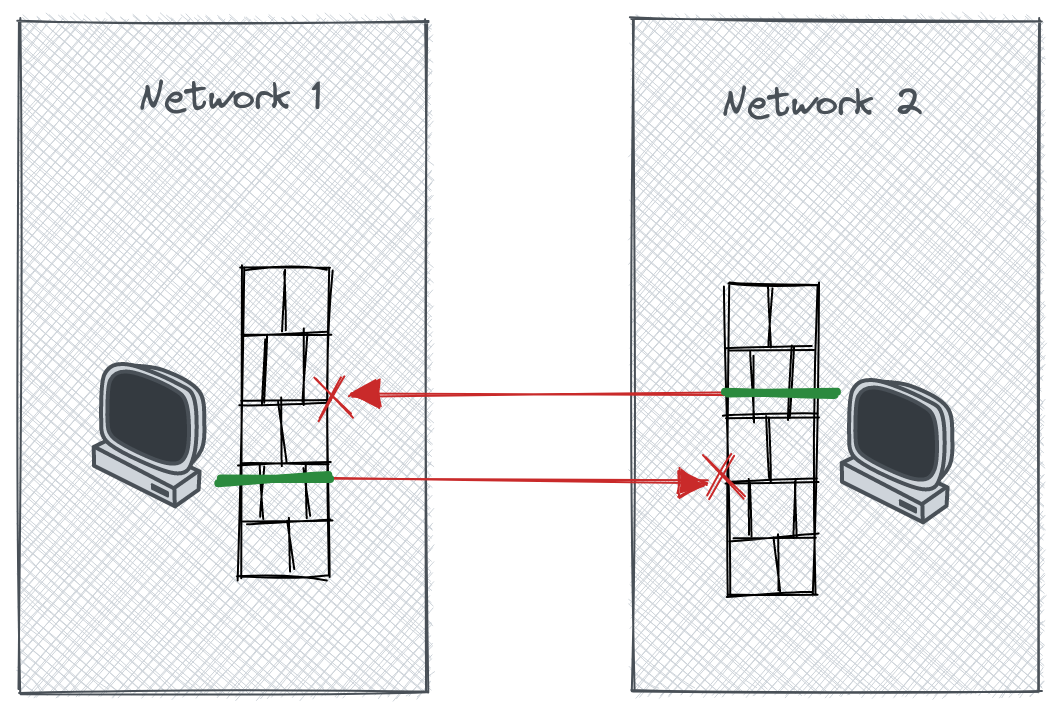
\includegraphics{../figures/nat-intro.png}

On the other hand, mesh \glspl{vpn} such as Tinc\autocite{tincDocs},
Tailscale\autocite{tailscaleDocs} and Nebula\autocite{nebulaDocs}
utilize direct \gls{p2p} links between the clients for the data traffic.
Authentication, authorization and traffic encryption are performed using
certificates based on public key cryptography. As we mentioned in the
introduction chapter, the devices in a typical home network can only
initiate connections to public endpoints (via \gls{nat}) but cannot be
discovered from outside their \gls{lan}. This poses a challenge when two
parties who want to communicate via a direct link are both behind
separate \glspl{nat} \ref{nat-intro} and neither can be contacted by the
other one first. Mesh \glspl{vpn} solve this issue via \gls{nat}
traversal techniques such as \gls{udp} hole punching based on concepts
from \gls{stun}. The machines of each party can contact a public
\gls{stun} server \ref{nat-traversal}, which will note what \gls{ip}
addresses the connections come from and inform the parties. Since the
parties initiated the connection to the STUN server, their routers will
keep a mapping between their local IP addresses and the port that was
allocated for the connection in order to be able to forward the incoming
traffic. Those ``holes'' in the NATs were originally intended for the
STUN server, but mesh VPNs use the stateless ``fire and forget'' UDP
protocol for their internal communication, which does not require nor
provides a mechanism for the NATs to verify who sent a UDP packet. With
most NATs, this is enough to be able to (ab)use the ``punched holes''
for the purpose of \gls{p2p} traffic from other parties. Mesh VPNs
implement the stateful \gls{tcp} and \gls{tls} protocols on top of UDP
and expose an regular network interface to the other programs, keeping
them shielded from the underlying complexities. Other NAT
implementations such as Symmetric NAT and \glspl{cgnat} can be more
difficult to ``punch through'' due to their more complex port mapping
strategies. In those cases, establishing P2P connections might involve
guess work or even fail and require falling back to routing the
(encrypted) traffic via another party or service.
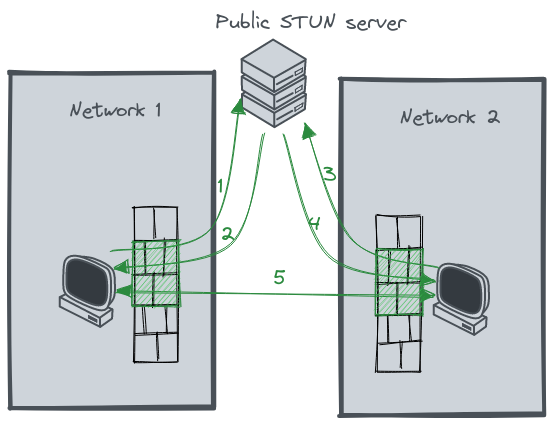
\includegraphics{../figures/nat-traversal.png}

Now that we have a general understanding of how mesh VPNs work, let us
see how Tinc, Tailscale and Nebula compare. All three are open-source,
with the exception of Tailscale's coordination service which handles the
peer discovery and identity management. Headscale
\autocite{fontJuanfontHeadscale2022} is a community driven open-source
alternative for that component. Tinc is the oldest of the three but has
a relatively small community. It is mainly developed by a single author
and appears to be more academic than industry motivated. Nebula and
Tailscale are both business driven. Tailscale was started by a number of
high profile ex-googlers and is the most end-user focused of the three,
providing a service that allows people to sign up using a variety of
identity providers including google, microsoft, github and others. They
also provide an Admin console that allows a user to easily add their
personal devices to a network or share them with others. It also has
support for automation tools like Terraform for creating authorization
keys and managing an \gls{acl} based firewall. Nebula was originally
developed at the instant messaging company Slack to create overlay
networks for their cross region cloud infrastructure, but the authors
later started a new company and are currently developing a user-centric
platform similar to Tailscale's. Nebula is more customizable than
Tailscale and since it is completely open-source it can be adapted to
different use cases, but it is also more involved to set up. A
certificate authority needs to be configured for issuing the identities
of the participating hosts. Furthermore, publicly accessible
coordination servers need to be deployed to facilitate the host
discovery. Tailscale employs a distributed relay network of \gls{derp}
servers, while Nebula can be configured to route via one of the other
peers in the VPN.

We decided to use Tailscale for the initial implementation of \gls{e3}
because it has all the necessary features to support networked MPC while
also being the easiest one to set up as it does not require any extra
services to be deployed.

We will now briefly mention some additional approaches we looked into
that may be a good starting point for the next phase of the project.

\hypertarget{decentralized-identifiers-dids-and-didcomm}{%
  \subsubsection{Decentralized Identifiers (DIDs) and
    DIDComm}\label{decentralized-identifiers-dids-and-didcomm}}

\gls{ssi} is a way of managing a digital identity that emphasises an
individual's ownerhip and control over their personal data. In contrast
with more traditional methods, SSI does not rely on a third party such
as a government or an organization to issue identities - people issue
their own identities, usually in the form of an asymmetric key-pair.
\glspl{did}\autocite{didW3C} are a form of \gls{ssi} that recently
reached W3C Recommendation Status and DIDComm\autocite{didcommSpec} is a
set of communication protocols based on DIDs. Its main design goals are
to be private, secure, decentralized, transport agnostic and routable.
Its primary concerns are with the message formats, cryptograhic
algorithms and processes that enable identity owners to find each other
and interact digitally based on their identities rather than TCP
concepts like IP addresses. One thing we noticed was that the initial
version of DIDComm does not support stateful sessions and therefore all
messages need to be both encrypted with the recepient's public key and
signed by the sender's private key. This will likely cause performance
issues in the MPC setting because it usually involves a large number of
small messages containing the secret shares of the parties. In order for
DIDComm to be usable for MPyC we would likely have to implement a
TLS-like protocol on top of it that supports sessions.

\hypertarget{the-onion-router-tor}{%
  \subsubsection{The Onion Router (TOR)}\label{the-onion-router-tor}}

Two machines need to know each other's IP addresses in order to be able
to interact via the internet. An IP address can reveal details about a
person's location or be used to launch a \gls{ddos} attack against them.
Additionally, nearby attackers could be listening to their traffic and
tracking their internet behaviour, which may be undesirable depending on
a person's privacy requirements. TOR uses a network of relays to
obfuscate the communication route between two parties. The original
sender prepares a multi-layered message, where each layer is encrypted
for a specific relayer. When one of them receives a message, they only
know who was the previous link and after decrypting their part of the
message, they know the next link. They do not know who was the original
sender and who is the final destination. The privacy comes at the cost
of performance. Additionally, TOR has the concept of Onion Services,
which receive an address under the .onion pseudo top level domain and
correspond to a public key
(e.g.~vww6ybal4bd7szmgncyruucpgfkqahzddi37ktceo3ah7ngmcopnpyyd.onion).
It allows two way privacy preserving communications. A concept similar
to TOR can be optionally incorporated in MPyC for the cases when privacy
is essential. It is interesting to measure the performance impact on
MPyC computations when routed via a TOR-like relay network.

\hypertarget{summary}{%
  \subsection{Summary}\label{summary}}

In this chapter we compared a number of potential building blocks for
\gls{e3} and made some choices informed by our requirements.
Specifically, we will use Terraform for provisioning Virtual Machines
running NixOS on DigitalOcean and Colmena for deploying to them. Our
initial implementation will use Tailscale as the connectivity layer due
to its ease of use. In the next phase of the project, we plan to explore
solutions based on Nebula, DIDComm, TOR and combinations of the above.

\hypertarget{design}{%
  \section{Design}\label{design}}

\hypertarget{section}{%
  \subsection{}\label{section}}

\hypertarget{implementation-details}{%
  \section{Implementation details}\label{implementation-details}}

In this chapter we will cover the implementation of \gls{e3}, which can
be found on \href{https://github.com/e-nikolov/mpyc}{Github}. It is a
fork of \href{https://github.com/lschoe/mpyc}{MPyC} that adds deployment
capabilities. We will now discuss the more critical parts of the
implementation.

\hypertarget{reproducible-development-of-mpyc}{%
  \subsection{Reproducible development of
    MPyC}\label{reproducible-development-of-mpyc}}

As previously discussed, the \glspl{vm} of \gls{e3} run the NixOS
distribution of Linux, which is based on the declarative package manager
Nix. One of its benefits is that it can also be used to declaratively
manage the dependencies of a software project via its development shells
feature. Normally such a project would have to explain in its readme how
to install and configure all of the extra tools that are needed for
working with it. On the other hand, with Nix, we can run the command
\texttt{nix\ develop} in a directory containing a declarative
specification in a flake.nix file. This will open a temporary shell
environment and install the specified versions of the dependencies.
Exiting the shell will uninstall them. This process makes it easy to
work on projects that require conflicting versions of packages. To
achieve this, nix does the following:

\begin{itemize}
  \tightlist
  \item
        it places each build result under \texttt{/nix/store/}, in a
        sub-directory prefixed by the hash of its inputs,
        e.g.~\texttt{/nix/store/2ispfz80kmwrsvwndxkxs56irn86h43p-bash-5.1-p16/}
  \item
        nix opens a new shell with a modified \texttt{PATH} environment
        variable that includes the nix store path that contains the new
        package.
\end{itemize}

There are tools like nix-direnv that take dev shells a step further by
automatically loading/unloading the specified dependencies when
entering/leaving a directory that contains a dev shell specification.

\newpage

The entrypoint for Nix in our MPyC fork is the
\href{https://github.com/e-nikolov/mpyc/blob/master/flake.nix}{flake.nix}
file. A simplified version can be seen below:

\begin{Shaded}
  \begin{Highlighting}[]

    \OperatorTok{\{}
    \VariableTok{description} \OperatorTok{=} \StringTok{"MPyC flake"}\OperatorTok{;}

    \VariableTok{inputs} \OperatorTok{=} \OperatorTok{\{}
    \VariableTok{nixpkgs}\NormalTok{.}\VariableTok{url} \OperatorTok{=} \StringTok{"github:nixos/nixpkgs/nixos{-}unstable"}\OperatorTok{;}
    \OperatorTok{\};}

    \VariableTok{outputs} \OperatorTok{=}\NormalTok{ inputs@}\OperatorTok{\{} \VariableTok{self}\OperatorTok{,} \VariableTok{nixpkgs}\OperatorTok{,} \OperatorTok{...} \OperatorTok{\}}\NormalTok{:}
    \KeywordTok{let}
    \CommentTok{\# import the derivation of mpyc and all of its python dependencies}
    \VariableTok{mpyc{-}demo} \OperatorTok{=} \OperatorTok{(}\BuiltInTok{import} \SpecialStringTok{./nix/mpyc{-}demo.nix} \OperatorTok{\{} \KeywordTok{inherit}\NormalTok{ pkgs}\OperatorTok{;} \VariableTok{dir} \OperatorTok{=} \SpecialStringTok{./.}\OperatorTok{;} \OperatorTok{\});}

    \VariableTok{pkgs} \OperatorTok{=} \BuiltInTok{import}\NormalTok{ nixpkgs }\OperatorTok{\{}
    \VariableTok{system} \OperatorTok{=} \StringTok{"x86\_64{-}linux"}\OperatorTok{;}
    \OperatorTok{\};}
    \KeywordTok{in}
    \OperatorTok{\{}
    \VariableTok{devShell}\NormalTok{.}\VariableTok{x86\_64{-}linux} \OperatorTok{=}\NormalTok{ pkgs.mkShell }\OperatorTok{\{}
    \VariableTok{shellHook} \OperatorTok{=} \StringTok{\textquotesingle{}\textquotesingle{}}
    \StringTok{          export PYTHONPATH=./}
    \StringTok{        \textquotesingle{}\textquotesingle{}}\OperatorTok{;}

    \VariableTok{nativeBuildInputs} \OperatorTok{=} \OperatorTok{[}
    \NormalTok{          pkgs.curl pkgs.jq}
    \NormalTok{          pkgs.colmena pkgs.pssh}
    \OperatorTok{(}\NormalTok{pkgs.terraform.withPlugins}
    \OperatorTok{(}\VariableTok{tp}\OperatorTok{:} \OperatorTok{[}
    \NormalTok{              tp.digitalocean tp.}\ConstantTok{null}
    \NormalTok{              tp.external tp.tailscale}
    \NormalTok{              tp.random}
    \OperatorTok{]))}
    \NormalTok{          mpyc{-}demo}
    \OperatorTok{];}
    \OperatorTok{\};}
    \OperatorTok{\};}
    \OperatorTok{\}}
  \end{Highlighting}
\end{Shaded}

The flake is functionally pure in the sense that all external inputs are
explicitly declared in the inputs section and their hashes are kept in a
\texttt{flake.lock} file. In our example, the only input is
\texttt{nixpkgs} - a community managed repository containing the nix
build expressions for more than 80 000 packages. When a nix command uses
the file for the first time, the latest revision of the nixos-unstable
branch of the git repository will be fetched and its contents will be
hashed and placed in the flake.lock. Further executions will reuse the
revision from the lock file and verify that the resulting hash matches
the original one. The lock file can be updated via the
\texttt{nix\ flake\ update} command. The output section contains the
\texttt{devShell.x86\_64-linux} attribute which declares the packages
required to work with the project. Specifically, it needs the nix
packages for curl, jq, colmena, pssh and terraform with a number of
plugins. Finally it also builds the \texttt{mpyc-demo} package which
contains python and all python dependencies needed by MPyC. Its
specification is imported from the \texttt{mpyc-demo.nix} file:

\begin{Shaded}
  \begin{Highlighting}[]
    \OperatorTok{\{} \VariableTok{pkgs}\OperatorTok{,} \VariableTok{dir} \OperatorTok{\}}\NormalTok{:}
    \OperatorTok{(}\NormalTok{pkgs.poetry2nix.mkPoetryEnv }\OperatorTok{\{}
    \VariableTok{python} \OperatorTok{=}\NormalTok{ pkgs.python3}\OperatorTok{;}
    \VariableTok{projectDir} \OperatorTok{=}\NormalTok{ dir}\OperatorTok{;}

    \VariableTok{extraPackages} \OperatorTok{=} \OperatorTok{(}\VariableTok{ps}\OperatorTok{:} \OperatorTok{[}
    \OperatorTok{(}\NormalTok{pkgs.python3Packages.buildPythonPackage}
    \OperatorTok{\{}
    \VariableTok{name} \OperatorTok{=} \StringTok{"mpyc"}\OperatorTok{;}
    \VariableTok{src} \OperatorTok{=}\NormalTok{ dir}\OperatorTok{;}
    \OperatorTok{\})}
    \OperatorTok{]);}

    \VariableTok{overrides} \OperatorTok{=}\NormalTok{ pkgs.poetry2nix.overrides.withDefaults }\OperatorTok{(}
    \VariableTok{self}\OperatorTok{:} \VariableTok{super}\OperatorTok{:} \OperatorTok{\{}
    \VariableTok{gmpy2} \OperatorTok{=}\NormalTok{ pkgs.python3Packages.gmpy2}\OperatorTok{;}
    \OperatorTok{\}}
    \OperatorTok{);}
    \OperatorTok{\})}
  \end{Highlighting}
\end{Shaded}

MPyC uses the python specific dependency management tool
poetry\autocite{poetryDocs} and the poetry2nix package dynamically
generates nix expressions from its configuration in
\texttt{pyproject.toml}

\begin{Shaded}
  \begin{Highlighting}[]
    \KeywordTok{[}\DataTypeTok{tool}\KeywordTok{.}\DataTypeTok{poetry}\KeywordTok{]}
    \DataTypeTok{name} \OperatorTok{=} \StringTok{"mpyc"}
    \DataTypeTok{version} \OperatorTok{=} \StringTok{"0.8.8"}
    \DataTypeTok{description} \OperatorTok{=} \StringTok{"MPyC for Multiparty Computation in Python"}
    \DataTypeTok{authors} \OperatorTok{=} \OperatorTok{[}\StringTok{"Berry Schoenmakers \textless{}berry@win.tue.nl\textgreater{}"}\OperatorTok{]}
    \DataTypeTok{readme} \OperatorTok{=} \StringTok{"README.md"}
    \DataTypeTok{packages} \OperatorTok{=} \OperatorTok{[\{}\DataTypeTok{include}\OperatorTok{ =} \StringTok{"demos"}\OperatorTok{\}]}

    \KeywordTok{[}\DataTypeTok{tool}\KeywordTok{.}\DataTypeTok{poetry}\KeywordTok{.}\DataTypeTok{dependencies}\KeywordTok{]}
    \DataTypeTok{python} \OperatorTok{=} \StringTok{"\^{}3.10"}
    \DataTypeTok{qrcode} \OperatorTok{=} \StringTok{"\^{}7.3.1"}
    \DataTypeTok{numpy} \OperatorTok{=} \StringTok{"\^{}1.23.4"}
    \DataTypeTok{gmpy2} \OperatorTok{=} \StringTok{"\^{}2.1.2"}

    \KeywordTok{[}\DataTypeTok{build{-}system}\KeywordTok{]}
    \DataTypeTok{requires} \OperatorTok{=} \OperatorTok{[}\StringTok{"poetry{-}core"}\OperatorTok{]}
    \DataTypeTok{build{-}backend} \OperatorTok{=} \StringTok{"poetry.core.masonry.api"}
  \end{Highlighting}
\end{Shaded}

There was an issue with the gmpy2 library when building it via
poetry2nix, but fortunately we could override it with the version
already present in nixpkgs.

Using this setup we can now go to the root directory of MPyC and run the
\texttt{nix\ develop} command, which will automatically download, build
and install all of our dependencies in a temporary shell. We are then
ready to make changes to MPyC or locally run the demos, e.g.~via
\texttt{python\ ./demos/secretsanta.py}. \#\# Building a NixOS image for
DigitalOcean As previously discussed we will deploy \gls{e3} on
DigitalOcean droplets - their name for \glspl{vm}. They do not provide
an official NixOS image, but we can build our own using nix.

\begin{Shaded}
  \begin{Highlighting}[]
    \CommentTok{\#\# flake.nix}

    \OperatorTok{\{}
    \VariableTok{inputs} \OperatorTok{=} \OperatorTok{\{}
    \VariableTok{nixpkgs}\NormalTok{.}\VariableTok{url} \OperatorTok{=} \StringTok{"github:nixos/nixpkgs/nixos{-}unstable"}\OperatorTok{;}
    \OperatorTok{\};}

    \VariableTok{outputs} \OperatorTok{=}\NormalTok{ inputs@}\OperatorTok{\{} \VariableTok{self}\OperatorTok{,} \VariableTok{nixpkgs}\OperatorTok{,} \OperatorTok{...} \OperatorTok{\}}\NormalTok{:}
    \KeywordTok{let}
    \VariableTok{mpyc{-}demo} \OperatorTok{=} \OperatorTok{(}\BuiltInTok{import} \SpecialStringTok{./nix/mpyc{-}demo.nix} \OperatorTok{\{} \KeywordTok{inherit}\NormalTok{ pkgs}\OperatorTok{;} \VariableTok{dir} \OperatorTok{=} \SpecialStringTok{./.}\OperatorTok{;} \OperatorTok{\});}

    \VariableTok{pkgs} \OperatorTok{=} \BuiltInTok{import}\NormalTok{ nixpkgs }\OperatorTok{\{}
    \VariableTok{system} \OperatorTok{=} \StringTok{"x86\_64{-}linux"}\OperatorTok{;}
    \OperatorTok{\};}

    \VariableTok{digitalOceanConfig} \OperatorTok{=} \BuiltInTok{import} \SpecialStringTok{./nix/digitalocean/image.nix} \OperatorTok{\{}
    \KeywordTok{inherit}\NormalTok{ pkgs}\OperatorTok{;}
    \VariableTok{extraPackages} \OperatorTok{=} \OperatorTok{[}\NormalTok{ mpyc{-}demo }\OperatorTok{];}
    \OperatorTok{\};}
    \KeywordTok{in}
    \OperatorTok{\{}
    \VariableTok{packages}\NormalTok{.}\VariableTok{digitalOceanImage} \OperatorTok{=} \OperatorTok{(}\NormalTok{pkgs.nixos digitalOceanConfig}\OperatorTok{)}\NormalTok{.digitalOceanImage}\OperatorTok{;}
    \OperatorTok{\};}
    \OperatorTok{\}}
  \end{Highlighting}
\end{Shaded}

\begin{Shaded}
  \begin{Highlighting}[]
    \CommentTok{\#\# nix/digitalocean/image.nix}

    \OperatorTok{\{} \VariableTok{pkgs}\OperatorTok{,} \VariableTok{extraPackages} \OperatorTok{?} \OperatorTok{[} \OperatorTok{],} \OperatorTok{...} \OperatorTok{\}}\NormalTok{:}
    \OperatorTok{\{}
    \VariableTok{imports} \OperatorTok{=} \OperatorTok{[} \StringTok{"}\SpecialCharTok{$\{}\NormalTok{pkgs.path}\SpecialCharTok{\}}\StringTok{/nixos/modules/virtualisation/digital{-}ocean{-}image.nix"} \OperatorTok{];}
    \VariableTok{system}\NormalTok{.}\VariableTok{stateVersion} \OperatorTok{=} \StringTok{"22.11"}\OperatorTok{;}

    \VariableTok{environment}\NormalTok{.}\VariableTok{systemPackages} \OperatorTok{=} \KeywordTok{with}\NormalTok{ pkgs}\OperatorTok{;} \OperatorTok{[}
    \NormalTok{    jq}
    \OperatorTok{]} \OperatorTok{++}\NormalTok{ extraPackages}\OperatorTok{;}

    \VariableTok{services}\NormalTok{.}\VariableTok{tailscale}\NormalTok{.}\VariableTok{enable} \OperatorTok{=} \ConstantTok{true}\OperatorTok{;}

    \VariableTok{networking}\NormalTok{.}\VariableTok{firewall} \OperatorTok{=} \OperatorTok{\{}
    \VariableTok{enable} \OperatorTok{=} \ConstantTok{true}\OperatorTok{;}
    \VariableTok{checkReversePath} \OperatorTok{=} \StringTok{"loose"}\OperatorTok{;}
    \VariableTok{trustedInterfaces} \OperatorTok{=} \OperatorTok{[} \StringTok{"tailscale0"} \OperatorTok{];}
    \OperatorTok{\};}
    \OperatorTok{\}}
  \end{Highlighting}
\end{Shaded}

The image is based on the default version provided by nixpkgs and adds
some extra packages and configurations. It:

\begin{itemize}
  \tightlist
  \item
        enables the tailscale service so that we can easily configure them to
        join the same tailscale network;
  \item
        configures the firewall to allow tailscale traffic;
  \item
        includes the \texttt{mpyc-demo} package we made earlier for the
        development shell.
\end{itemize}

The image will likely be built only once, but it is still useful to have
even an outdated version of the demo baked into it as it helps us avoid
having to build all of the python dependencies while deploying later.

Running \texttt{nix\ build\ .\#packages.digitalOceanImage} creates a
\texttt{.qcow2.gz} formatted image file that can be imported into
DigitalOcean.

\hypertarget{building-a-nixos-image-for-raspberrypi}{%
  \subsection{Building a NixOS image for
    RaspberryPi}\label{building-a-nixos-image-for-raspberrypi}}

We can build a NixOS image for a RaspberryPi4 with a similar nix
expression:

\begin{Shaded}
  \begin{Highlighting}[]
    \OperatorTok{\{}
    \VariableTok{inputs} \OperatorTok{=} \OperatorTok{\{}
    \VariableTok{nixpkgs}\NormalTok{.}\VariableTok{url} \OperatorTok{=} \StringTok{"github:nixos/nixpkgs/nixos{-}unstable"}\OperatorTok{;}
    \OperatorTok{\};}

    \VariableTok{outputs} \OperatorTok{=}\NormalTok{ inputs@}\OperatorTok{\{} \VariableTok{self}\OperatorTok{,} \VariableTok{nixpkgs}\OperatorTok{,} \OperatorTok{...} \OperatorTok{\}}\NormalTok{:}
    \KeywordTok{let}
    \VariableTok{mpyc{-}demo} \OperatorTok{=} \OperatorTok{(}\BuiltInTok{import} \SpecialStringTok{./nix/mpyc{-}demo.nix} \OperatorTok{\{} \KeywordTok{inherit}\NormalTok{ pkgs}\OperatorTok{;} \VariableTok{dir} \OperatorTok{=} \SpecialStringTok{./.}\OperatorTok{;} \OperatorTok{\});}

    \VariableTok{pkgs} \OperatorTok{=} \BuiltInTok{import}\NormalTok{ nixpkgs }\OperatorTok{\{}
    \VariableTok{system} \OperatorTok{=} \StringTok{"aarch64{-}linux"}\OperatorTok{;}
    \OperatorTok{\};}
    \KeywordTok{in}
    \OperatorTok{\{}
    \VariableTok{packages}\NormalTok{.}\VariableTok{raspberryPi4Image} \OperatorTok{=} \OperatorTok{(}\NormalTok{pkgs.nixos }\OperatorTok{(\{} \VariableTok{config}\OperatorTok{,} \OperatorTok{...} \OperatorTok{\}}\NormalTok{: }\OperatorTok{\{}
    \VariableTok{system}\NormalTok{.}\VariableTok{stateVersion} \OperatorTok{=} \StringTok{"22.11"}\OperatorTok{;}
    \VariableTok{imports} \OperatorTok{=} \OperatorTok{[}
    \OperatorTok{(}\StringTok{"}\SpecialCharTok{$\{}\NormalTok{pkgs.path}\SpecialCharTok{\}}\StringTok{/nixos/modules/installer/sd{-}card/sd{-}image{-}aarch64{-}installer.nix"}\OperatorTok{)}
    \OperatorTok{];}

    \VariableTok{environment}\NormalTok{.}\VariableTok{systemPackages} \OperatorTok{=} \OperatorTok{[}
    \NormalTok{                mpyc{-}demo}
    \OperatorTok{];}
    \OperatorTok{\}))}\NormalTok{.sdImage}\OperatorTok{;}
    \OperatorTok{\};}
    \OperatorTok{\}}
  \end{Highlighting}
\end{Shaded}

The build command has to be executed on an ARM64 based processor in
order to succeed. This can be achieved either via emulation with qemu
binfmt or via a virtual machine. When already running NixOS as a host,
all that is required is to add
\texttt{extra-platforms\ =\ aarch64-linux} to the
\texttt{/etc/nixos/nix.conf} file. \#\# Provisioning via Terraform We
will provision DigitalOcean droplets with Terraform from the VM image
created earlier. We need to provide it with a DigitalOcean authorization
key in the \texttt{DIGITALOCEAN\_TOKEN} environment variable so it can
use their API on our behalf.

\hypertarget{importing-the-image}{%
  \paragraph{Importing the image}\label{importing-the-image}}

The snippet below handles the upload of our NixOS image.

\begin{Shaded}
  \begin{Highlighting}[]
    \NormalTok{variable "nixos{-}image{-}path" \{}
    \NormalTok{  type    = string}
    \NormalTok{  default = "../../bin/image/nixos.qcow2.gz"}
    \NormalTok{\}}

    \NormalTok{resource "digitalocean\_spaces\_bucket" "tf{-}state" \{}
    \NormalTok{  name   = "mpyc{-}tf{-}state"}
    \NormalTok{  region = "ams3"}

    \NormalTok{  lifecycle \{}
    \NormalTok{    prevent\_destroy = true}
    \NormalTok{  \}}
    \NormalTok{\}}

    \NormalTok{resource "digitalocean\_spaces\_bucket\_object" "nixos{-}image" \{}
    \NormalTok{  region = digitalocean\_spaces\_bucket.tf{-}state.region}
    \NormalTok{  bucket = digitalocean\_spaces\_bucket.tf{-}state.name}
    \NormalTok{  key    = basename(var.nixos{-}image{-}path)}
    \NormalTok{  source = var.nixos{-}image{-}path}
    \NormalTok{  acl    = "public{-}read"}
    \NormalTok{  etag   = filemd5(var.nixos{-}image{-}path)}
    \NormalTok{\}}

    \NormalTok{resource "digitalocean\_custom\_image" "nixos{-}image" \{}
    \NormalTok{  name    = "nixos{-}22.11"}
    \NormalTok{  url     = "https://$\{digitalocean\_spaces\_bucket.tf{-}state.bucket\_domain\_name\}/$\{digitalocean\_spaces\_bucket\_object.nixos{-}image.key\}"}
    \NormalTok{  regions = local.all\_regions}
    \NormalTok{  tags    = ["nixos"]}

    \NormalTok{  lifecycle \{}
    \NormalTok{    replace\_triggered\_by = [}
    \NormalTok{      digitalocean\_spaces\_bucket\_object.nixos{-}image}
    \NormalTok{    ]}
    \NormalTok{  \}}
    \NormalTok{\}}
  \end{Highlighting}
\end{Shaded}

The DigitalOcean API only supports importing images from a URL, so we
first need to upload the image to a publicly accessible location. For
that purpose, the snippet above first provisions a Bucket within Spaces
- DigitalOcean's cloud storage solution and uploads the image there.
After that, the \texttt{digitalocean\_custom\_image} will import the
image from the URL generated by the bucket.

\hypertarget{generating-hostnames}{%
  \paragraph{Generating hostnames}\label{generating-hostnames}}

The snippet below starts with a specification of how many machines per
region we want to have and transforms it into a list of descriptive ids
(e.g.~\texttt{mpyc-demo-\/-ams3-0-15e53f39}) that will be used as host
names so we can easily distinguish the machines when they start
communicating with each other.

\begin{Shaded}
  \begin{Highlighting}[]
    \NormalTok{locals \{}
    \NormalTok{  node\_definitions = var.DESTROY\_NODES != "" ? [}
    \NormalTok{    \{ region = "ams3", num = 0 \},}
    \NormalTok{    \{ region = "sfo3", num = 0 \},}
    \NormalTok{    \{ region = "nyc3", num = 0 \},}
    \NormalTok{    \{ region = "sgp1", num = 0 \},}
    \NormalTok{    ] : [}
    \NormalTok{    \{ region = "ams3", num = 3 \},}
    \NormalTok{    \{ region = "sfo3", num = 1 \},}
    \NormalTok{    \{ region = "nyc3", num = 1 \},}
    \NormalTok{    \{ region = "sgp1", num = 1 \},}
    \NormalTok{  ]}

    \NormalTok{  nodes\_expanded = flatten([}
    \NormalTok{    for node in local.node\_definitions : [}
    \NormalTok{      for i in range(node.num) :}
    \NormalTok{      merge(node, \{}
    \NormalTok{        name = "mpyc{-}demo{-}{-}$\{node.region\}{-}$\{i\}"}
    \NormalTok{      \})}
    \NormalTok{    ]}
    \NormalTok{  ])}

    \NormalTok{  nodes = \{}
    \NormalTok{    for node in local.nodes\_expanded :}
    \NormalTok{    node.name =\textgreater{} merge(node, \{}
    \NormalTok{      hostname = "$\{node.name\}{-}$\{random\_id.mpyc{-}node{-}hostname[node.name].hex\}"}
    \NormalTok{    \})}
    \NormalTok{  \}}
    \NormalTok{\}}
  \end{Highlighting}
\end{Shaded}

\hypertarget{provisioning-the-hosts}{%
  \paragraph{Provisioning the hosts}\label{provisioning-the-hosts}}

The snippet below provisions the droplets in the specified regions and
then using Tailscale's terraform provider creates auth keys for the
machines, copies them to the machines and configures them to join the
tailscale network. When the droplets are being destroyed, the
provisioner will remove the nodes from the network.

\begin{Shaded}
  \begin{Highlighting}[]
    \NormalTok{resource "digitalocean\_droplet" "mpyc{-}node" \{}
    \NormalTok{  for\_each = local.nodes}

    \NormalTok{  image    = digitalocean\_custom\_image.nixos{-}image.id}
    \NormalTok{  name     = each.value.hostname}
    \NormalTok{  region   = each.value.region}
    \NormalTok{  size     = "s{-}1vcpu{-}1gb"}
    \NormalTok{  ssh\_keys = [for key in digitalocean\_ssh\_key.ssh{-}keys : key.fingerprint]}

    \NormalTok{  connection \{}
    \NormalTok{    type = "ssh"}
    \NormalTok{    user = "root"}
    \NormalTok{    host = self.ipv4\_address}
    \NormalTok{  \}}

    \NormalTok{  provisioner "remote{-}exec" \{}
    \NormalTok{    inline = [}
    \NormalTok{      "mkdir {-}p /var/keys/",}
    \NormalTok{      "echo $\{tailscale\_tailnet\_key.keys.key\} \textgreater{} /var/keys/tailscale",}
    \NormalTok{      "tailscale up {-}{-}auth{-}key file:/var/keys/tailscale"}
    \NormalTok{    ]}
    \NormalTok{  \}}

    \NormalTok{  provisioner "remote{-}exec" \{}
    \NormalTok{    when = destroy}
    \NormalTok{    inline = [}
    \NormalTok{      "tailscale logout"}
    \NormalTok{    ]}
    \NormalTok{  \}}

    \NormalTok{  lifecycle \{}
    \NormalTok{    replace\_triggered\_by = [}
    \NormalTok{      tailscale\_tailnet\_key.keys}
    \NormalTok{    ]}
    \NormalTok{  \}}
    \NormalTok{\}}

    \NormalTok{resource "tailscale\_tailnet\_key" "keys" \{}
    \NormalTok{  reusable      = true}
    \NormalTok{  ephemeral     = true}
    \NormalTok{  preauthorized = true}
    \NormalTok{\}}
  \end{Highlighting}
\end{Shaded}

\hypertarget{interfacing-with-other-tools}{%
  \paragraph{Interfacing with other
    tools}\label{interfacing-with-other-tools}}

This snippet outputs the hostnames of the provisioned droplets so they
can be picked up by other tools. For example Colmena will read them from
a json file so it can deploy further software changes to them.

\begin{Shaded}
  \begin{Highlighting}[]


    \NormalTok{output "hosts{-}colmena" \{}
    \NormalTok{  value = \{ for node in local.nodes : node.hostname =\textgreater{} \{\} \}}
    \NormalTok{\}}

    \NormalTok{output "hosts{-}pssh" \{}
    \NormalTok{  value = join("", [for node in local.nodes : "root@$\{node.hostname\}\textbackslash{}n"])}
    \NormalTok{\}}
  \end{Highlighting}
\end{Shaded}

\hypertarget{colmena-deployment}{%
  \subsection{Colmena deployment}\label{colmena-deployment}}

Whenever we need to update the NixOS configuration of our VMs, we could
rebuild the image and re-provision them, but this would be slow. Instead
we use Colmena to deploy and apply the new configuration to all existing
VMs. It uses the same \texttt{digitalOceanConfig} attribute we created
for the NixOS image:

\begin{Shaded}
  \begin{Highlighting}[]
    \OperatorTok{\{}
    \VariableTok{inputs} \OperatorTok{=} \OperatorTok{\{}
    \VariableTok{nixpkgs}\NormalTok{.}\VariableTok{url} \OperatorTok{=} \StringTok{"github:nixos/nixpkgs/nixos{-}unstable"}\OperatorTok{;}
    \OperatorTok{\};}

    \VariableTok{outputs} \OperatorTok{=}\NormalTok{ inputs@}\OperatorTok{\{} \VariableTok{self}\OperatorTok{,} \VariableTok{nixpkgs}\OperatorTok{,} \OperatorTok{...} \OperatorTok{\}}\NormalTok{:}
    \KeywordTok{let}
    \VariableTok{mpyc{-}demo} \OperatorTok{=} \OperatorTok{(}\BuiltInTok{import} \SpecialStringTok{./nix/mpyc{-}demo.nix} \OperatorTok{\{} \KeywordTok{inherit}\NormalTok{ pkgs}\OperatorTok{;} \VariableTok{dir} \OperatorTok{=} \SpecialStringTok{./.}\OperatorTok{;} \OperatorTok{\});}

    \VariableTok{pkgs} \OperatorTok{=} \BuiltInTok{import}\NormalTok{ nixpkgs }\OperatorTok{\{}
    \VariableTok{system} \OperatorTok{=} \StringTok{"x86\_64{-}linux"}\OperatorTok{;}
    \OperatorTok{\};}

    \VariableTok{digitalOceanConfig} \OperatorTok{=} \BuiltInTok{import} \SpecialStringTok{./nix/digitalocean/image.nix} \OperatorTok{\{}
    \KeywordTok{inherit}\NormalTok{ pkgs}\OperatorTok{;}
    \VariableTok{extraPackages} \OperatorTok{=} \OperatorTok{[}\NormalTok{ mpyc{-}demo }\OperatorTok{];}
    \OperatorTok{\};}
    \KeywordTok{in}
    \OperatorTok{\{}
    \VariableTok{packages}\NormalTok{.}\VariableTok{colmena} \OperatorTok{=} \OperatorTok{\{}
    \VariableTok{meta} \OperatorTok{=} \OperatorTok{\{}
    \VariableTok{nixpkgs} \OperatorTok{=}\NormalTok{ pkgs}\OperatorTok{;}
    \OperatorTok{\};}
    \VariableTok{defaults} \OperatorTok{=}\NormalTok{ digitalOceanConfig}\OperatorTok{;}
    \OperatorTok{\}} \OperatorTok{//} \BuiltInTok{builtins}\NormalTok{.fromJSON }\OperatorTok{(}\BuiltInTok{builtins}\NormalTok{.readFile }\SpecialStringTok{./hosts.json}\OperatorTok{);}
    \OperatorTok{\};}
    \OperatorTok{\}}
  \end{Highlighting}
\end{Shaded}

This allows us to quickly make changes to the NixOS configuration,
deploy it via Colmena and once we are satisfied with it, we can choose
to rebuild the image so that new machines get provisioned with all of
our changes baked in.

\hypertarget{runtime-execution}{%
  \subsection{Runtime execution}\label{runtime-execution}}

We have identified the tools we will use to deploy \gls{e3} and how the
host machines will communicate. What remains is to determine how to run
a joint computation on the hosts. When running such an experiment, it
would be desirable to be able to iterate quickly. Colmena can be used to
deploy a new version of the whole operating system, but it would be
unnecessary to rebuild all dependencies every time we want to run a
command. Therefore we decided to use two additional tools:

\begin{itemize}
  \tightlist
  \item
        \emph{prsync} - a variant of the popular \emph{rsync} utility that can
        additively sync the contents of a directory to multiple remote hosts
  \item
        \emph{pssh} - a tool for executing an ssh command on many hosts in
        parallel
\end{itemize}

An example execution looks like this:

\begin{Shaded}
  \begin{Highlighting}[]
    \ExtensionTok{prsync} \AttributeTok{{-}h}\NormalTok{ hosts.pssh }\AttributeTok{{-}zarv} \AttributeTok{{-}p}\NormalTok{ 4 ./ /root/mpyc}
    \ExtensionTok{pssh} \AttributeTok{{-}h}\NormalTok{ hosts.pssh }\AttributeTok{{-}iv} \AttributeTok{{-}o}\NormalTok{ ./logs/}\VariableTok{$t} \StringTok{"cd /root/mpyc \&\& ./prun.sh"}
  \end{Highlighting}
\end{Shaded}

It loads the hostnames from the \texttt{hosts.pssh} file that was
previously generated by terraform and syncs the current state of the
mpyc directory. The second line will execute the \texttt{prun.sh} script
on each host.

An example of a possible \texttt{prun.sh} script:

\begin{Shaded}
  \begin{Highlighting}[]
    \CommentTok{\#!/bin/sh}

    \VariableTok{MAX\_PARTIES}\OperatorTok{=}\NormalTok{600}
    \VariableTok{hosts}\OperatorTok{=}\StringTok{"./hosts.pssh"}
    \VariableTok{port}\OperatorTok{=}\NormalTok{11599}

    \VariableTok{i}\OperatorTok{=}\NormalTok{0}
    \VariableTok{MY\_PID}\OperatorTok{=}\NormalTok{{-}1}

    \VariableTok{args}\OperatorTok{=}\StringTok{""}
    \ControlFlowTok{while} \VariableTok{IFS}\OperatorTok{=} \BuiltInTok{read} \AttributeTok{{-}r} \VariableTok{line}
    \ControlFlowTok{do}
    \ControlFlowTok{if} \BuiltInTok{[} \VariableTok{$i} \OtherTok{{-}ge} \VariableTok{$MAX\_PARTIES} \BuiltInTok{]}
    \ControlFlowTok{then}
    \ControlFlowTok{break}
    \ControlFlowTok{fi}
    \ControlFlowTok{if} \BuiltInTok{[} \OtherTok{{-}z} \StringTok{"}\VariableTok{$line}\StringTok{"} \BuiltInTok{]}
    \ControlFlowTok{then}
    \ControlFlowTok{break}
    \ControlFlowTok{fi}

    \VariableTok{host}\OperatorTok{=}\VariableTok{$\{line}\OperatorTok{\#}\StringTok{"root@"}\VariableTok{\}}

    \ControlFlowTok{if} \BuiltInTok{[} \StringTok{"}\VariableTok{$host}\StringTok{"} \OtherTok{=} \StringTok{"}\VariableTok{$HOSTNAME}\StringTok{"} \BuiltInTok{]}
    \ControlFlowTok{then}
    \VariableTok{MY\_PID}\OperatorTok{=}\VariableTok{$i}
    \ControlFlowTok{fi}
    \KeywordTok{((}\VariableTok{i} \OperatorTok{=} \VariableTok{i} \OperatorTok{+} \DecValTok{1}\KeywordTok{))}

    \VariableTok{args}\OperatorTok{+=}\StringTok{" {-}P }\VariableTok{$host}\StringTok{:}\VariableTok{$port}\StringTok{"}
    \ControlFlowTok{done} \OperatorTok{\textless{}} \StringTok{"}\VariableTok{$hosts}\StringTok{"}

    \ControlFlowTok{if} \BuiltInTok{[} \VariableTok{$MY\_PID} \OtherTok{=}\NormalTok{ {-}1 }\BuiltInTok{]}
    \ControlFlowTok{then}
    \BuiltInTok{echo}\NormalTok{ Only }\VariableTok{$i}\NormalTok{ parties are allowed. }\VariableTok{$HOSTNAME}\NormalTok{ will not participate in this MPC session}
    \ControlFlowTok{else}

    \VariableTok{cmd}\OperatorTok{=}\StringTok{"python ./demos/secretsanta.py 3 {-}{-}log{-}level debug }\DataTypeTok{\textbackslash{}}
    \StringTok{    {-}I }\VariableTok{$\{MY\_PID\}}\StringTok{ }\DataTypeTok{\textbackslash{}}
    \StringTok{    }\VariableTok{$\{args\}}\StringTok{"}

    \BuiltInTok{echo} \VariableTok{$cmd}
    \VariableTok{$cmd}

    \ControlFlowTok{fi}
  \end{Highlighting}
\end{Shaded}

Each host runs the same script that builds the arguments for the
\texttt{secretsanta.py} demo of MPyC. Each party determines its own
Party ID based on the index at which its hostname appears in the
\texttt{hosts.pssh} file.

\hypertarget{secrets}{%
  \subsection{Secrets}\label{secrets}}

The implementation expects that secrets are supplied as environment
variables with the specific mechanism being left up to the user. We are
currently keeping the secret values in the 1Password manager and use its
\gls{cli} to populate the environment variables at runtime, e.g.~via
\texttt{op\ run\ -\/-\ make\ deploy}.

\hypertarget{conclusions}{%
  \section{Conclusions}\label{conclusions}}

In this report we presented the results of the preparation phase for the
master thesis assignment ``Secure Sessions for Ad Hoc Multiparty
Computation in MPyC''. We developed an \acrfull{e3} for the purpose of
creating ad hoc networks of host machines that perform \acrfullpl{mpc}
in hybrid scenarios involving both cloud and physical machines. \gls{e3}
makes extensive use of declarative \gls{iac} tools in order to achieve
highly reproducible deployments in an automated way. We provided a
reference implementation that makes use of the Tailscale mesh VPN that
creates a network of RaspberryPis and cloud \glspl{vm} on DigitalOcean.
The cloud provisioning is defined declaratively using Terraform and
allows to define a set of host machines across the regions supported by
DigitalOcean (e.g.~Amsterdam, New York City, etc) and automatically add
them to a shared Tailscale network. The machines run NixOS - a
declarative and highly reproducible Linux distribution while Colmena is
used to declaratively manage the software installed on them via
\gls{ssh}. The tools \texttt{prsync} and \texttt{pssh} are used to run
MPyC demos in parallel on the deployed hosts.

\hypertarget{implementation-phase-planning}{%
  \paragraph{Implementation phase
    planning}\label{implementation-phase-planning}}

During the next phase of the thesis assignment, we plan to implement
various connectivity approaches for \gls{e3}'s host machines and analyse
their suitability for MPyC.

The following is a list of high level tasks that we plan to carry out as
part of the implementation phase:

\begin{itemize}
  \item
        replace the proprietary Tailscale coordination service from our
        reference implementation of \gls{e3} with the open-source self-hosted
        alternative Headscale\autocite{fontJuanfontHeadscale2022}
  \item
        develop a network overlay for \gls{e3} based on the Nebula mesh VPN.
        Nebula only provides a way to manually perform the initial setup, so
        our implementation should add a way to automatically:

        \begin{itemize}
          \tightlist
          \item
                allocate virtual IP addresses for the hosts
          \item
                generate identity certificates using the Nebula \gls{ca}
          \item
                distribute the certificates among the hosts
        \end{itemize}
  \item
        develop network overlays for \gls{e3} that incorporate parts of the
        mesh VPN implementations but with alternative identity management
        approaches:

        \begin{itemize}
          \tightlist
          \item
                using a \gls{ca} that is managed jointly using MPC
          \item
                using a form of \gls{ssi} such as \glspl{did}
        \end{itemize}
  \item
        implement a network overlay for \gls{e3} based on DIDComm
  \item
        explore options for enhancing the DIDComm implementation to:

        \begin{itemize}
          \tightlist
          \item
                support sessions - the DIDComm protocol is currently stateless and
                uses a new asymmetric key for each message, which negatively impacts
                performance
          \item
                employ \gls{nat} traversal techniques similar to mesh \glspl{vpn}
        \end{itemize}
  \item
        implement a privacy mechanism for \gls{e3} based on \gls{tor} in order
        to prevent leaking sensitive information like which parties are
        communicating with each other and their IP addresses
  \item
        investigate if we can apply ideas from the \gls{p2p} implementations
        in other software like the
        Ethereum{[}\textcite{ethereumDocs}{]}\autocite{ethereumYellowPaper}
        blockchain and the \gls{ipfs} \autocite{ipfsDocs}
  \item
        analyse and compare all of the above implementations in terms of:

        \begin{itemize}
          \tightlist
          \item
                security
          \item
                performance
          \item
                ease of use
          \item
                privacy
        \end{itemize}
  \item
        compare \gls{e3} to other work related to deploying MPC such as the
        Carbyne stack\autocite{robertboschgmbhCarbyneStack2022}
  \item
        references

        \begin{itemize}
          \tightlist
          \item[$\boxtimes$]
            don't cite tcp/ip
          \item[$\square$]
            Don't cite assorted mpc algorithms

            \begin{itemize}
              \tightlist
              \item
                    Write something like ``A good itroduction to MPC can be found on
                    WIkipedia {[}cite{]}, while an assortment of MPC techniques is
                    presented indepth by {[}assorted{]}''
            \end{itemize}
          \item
                Blue links
        \end{itemize}
  \item
        requirements -\textgreater{} goals/objectives
  \item
        Title -\textgreater{} Secure Sessions for Ad Hoc Multiparty
        Computation in MPyC
  \item
        e\^{}3? evaluation?
  \item
        remove the footers
  \item
        something with the abreviations
  \item
        proof read

        \begin{itemize}
          \tightlist
          \item
                check for things like we've
        \end{itemize}
  \item
        Intro

        \begin{itemize}
          \tightlist
          \item
                what is this project?
          \item
                what is mpc
          \item
                what is mpyc
          \item
          \item
                research questions
        \end{itemize}
  \item
        Demo

        \begin{itemize}
          \tightlist
          \item
                provisioning with terraform
          \item
                run an mpc demo
          \item
                destruction of the infra
        \end{itemize}
\end{itemize}

\printbibliography

\end{document}
